A simplified pipeline was modelled, based on typical off-shore pipelines that transport gas from Norway to Europe. The simplified pipeline profile is illustrated in \cref{fig:illustrationOfSimplifiedPipeline}, and the pipe wall composition in \cref{fig:pipeCrossSection}.

% \begin{figure}[ht]%
%     \centering%
%     \import{figures/}{simplified_pipeline_illustration04.pdf_tex}%
%     \caption{%
%         Illustration of the simplified pipeline. The pipe is onshore and buried 2~m underground for the first and last 25~km, and 100~m below sea level and exposed to sea water for 600~km between the onshore sections. Figure created freely after figure in \cite{Helgaker2013Modeling}.
%         \label{fig:illustrationOfSimplifiedPipeline}%
%     }%
% \end{figure}%

% \begin{figure}[ht]%
%     \centering%
%     \import{figures/}{pipe_cross_section03_rotated.pdf_tex}%
%     \caption{%
%         Illustration of pipe and pipe wall materials. The model pipeline has an inner diameter of \SI{1}{\meter}, and the pipe wall consists of \SI{24}{mm} of steel, coated with \SI{7}{mm} of a protective asphalt coating, and finally \SI{80}{mm} of concrete.
%         \label{fig:pipeCrossSection}%
%     }%
% \end{figure}%

\begin{figure}[!ht]%
\centering%
\begin{minipage}{9.6cm}%
    \import{figures/}{simplified_pipeline_illustration04.pdf_tex}%
    \\ % add newline so caption ends up below fig. 1, instead of messed up
    \parbox{0.9\textwidth}{%
        \vspace{2mm}%
        \caption{%
            Illustration of the simplified pipeline. The pipe is on-shore and buried 2~m underground for the first and last 25~km, and 100~m below sea level and exposed to sea water for 600~km between the on-shore sections. Figure created freely after figure in \cite{Helgaker2013Modeling}.%
            \label{fig:illustrationOfSimplifiedPipeline}%
        }%
    }%
\end{minipage}%
\hspace{0.099cm}%
\begin{minipage}{6.3cm}%
    \import{figures/}{pipe_cross_section03_rotated.pdf_tex}%
    \caption{%
        Illustration of pipe and pipe wall materials. The model pipeline has an inner diameter of \SI{1}{\meter}, and the pipe wall consists of \SI{24}{mm} of steel, coated with \SI{7}{mm} of a protective asphalt coating, and finally \SI{80}{mm} of concrete.%
        \label{fig:pipeCrossSection}%
    }%
\end{minipage}%
\end{figure}

The pipeline has an inner diameter of \SI{1}{\meter}, and consists of a steel pipeline, coated with a protective asphalt coating, and an outer concrete shell. The pipeline is on-shore and buried underground for the first \SI{25}{\kilo\meter}. It is then \SI{100}{\meter} below sea level and exposed to sea water for \SI{600}{\kilo\meter}, before it is on-shore and buried for the final \SI{25}{\kilo\meter}.

\subsubsection{Boundary conditions}
The boundary conditions for the pipeline was constant inlet temperature of \SI{33}{\degreeCelsius}, constant outlet pressure of 10 MPa, and constant air and sea water temperatures of respectively \SI{6}{\degreeCelsius} and \SI{4}{\degreeCelsius}. The system was thermalized with constant inlet mass flow of \SI{600}{\kg\per\second}, and then the mass flow rate was gradually decreased from \SI{600}{\kg\per\second} to \SI{200}{\kg\per\second} in a span of 4 minutes to emulate a transient. The mass flow transient is shown in \cref{fig:massFlowBoundaryCondition}. These conditions correspond to a Reynolds number of 40 to 50 million.

\begin{figure}[ht]%
    \centering%
    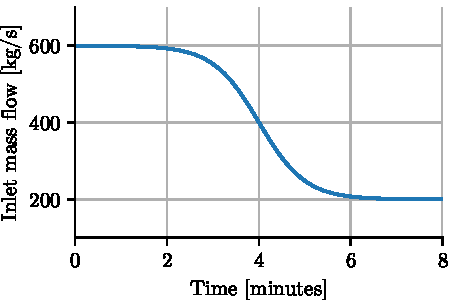
\includegraphics{figures/inlet_mass_flow.pdf}%
    \caption{%
        Plot of the inlet mass flow boundary condition, which simulates a transient occuring in a time span of approx 4~minutes.
        \label{fig:massFlowBoundaryCondition}%
    }%
\end{figure}%

% \begin{figure}[!ht]%
% \centering%
% \begin{minipage}{9.6cm}%
%     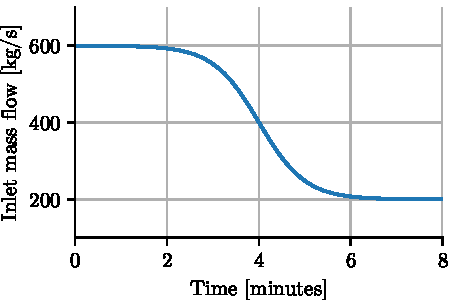
\includegraphics{figures/inlet_mass_flow.pdf}%
%     \caption{%
%         Plot of the inlet mass flow boundary condition, which simulates a transient occuring in a time span of approx 4~minutes.%
%         \label{fig:massFlowBoundaryCondition}%
%     }%
% \end{minipage}%
% \hspace{0.099cm}%
% \begin{minipage}{6.3cm}%
%     \caption{%
%         The gas.  composition used for the simulations.%
%         \label{tab:composition}%
%     }%
%     % \begin{tabular}{lc}
%     % \centering
%     % \begin{tabular}{lS}
%     \begin{tabular}{cl}%
%         \toprule
%         Component & {Mole fraction} \\ % use braces to protect from siunitx "S" alignment
%         \midrule
%         CH$_4$ & 0.8916 \\
%         C$_2$H$_6$ & 0.073513 \\
%         C$_3$H$_8$ & 0.005104 \\
%         iC$_4$H$_{10}$ & 0.000251 \\
%         nC$_4$H$_{10}$ & 0.000311 \\
%         iC$_5$H$_{12}$ & 0.000009 \\
%         nC$_5$H$_{12}$ & 0.000024 \\
%         N$_2$ & 0.006980 \\
%         CO$_2$ & 0.022208 \\
%         \bottomrule%
%     \end{tabular}
% \end{minipage}%
% \end{figure}%


The gas composition was kept fixed at the values shown in \cref{tab:composition}.
\begin{table}[!hb]
    \caption{
        The gas.  composition used for the simulations.
        \label{tab:composition}
    }
    % \begin{tabular}{lc}
    \centering
    % \begin{tabular}{lS}
    \begin{tabular}{cl}
        \toprule
        Component & {Mole fraction} \\ % use braces to protect from siunitx "S" alignment
        \midrule
        CH$_4$ & 0.8916 \\
        C$_2$H$_6$ & 0.073513 \\
        C$_3$H$_8$ & 0.005104 \\
        iC$_4$H$_{10}$ & 0.000251 \\
        nC$_4$H$_{10}$ & 0.000311 \\
        iC$_5$H$_{12}$ & 0.000009 \\
        nC$_5$H$_{12}$ & 0.000024 \\
        N$_2$ & 0.006980 \\
        CO$_2$ & 0.022208 \\
        \bottomrule
    \end{tabular}
\end{table}
%
% \begin{table}
%     \caption{
%         \redtext{Caption}
%         % \label{tab:composition}
%     }
%     \centering
%     \begin{tabular}{llllllllll}
%         \toprule
%         Component & CH$_4$ & C$_2$H$_6$ & C$_3$H$_8$ & iC$_4$H$_{10}$ &nC$_4$H$_{10}$ & iC$_5$H$_{12}$ & nC$_5$H$_{12}$ & N$_2$ & CO$_2$ \\
%         Mole fraction & 89.16 & 7.35 & 0.510 & 0.0251 & 0.0311 & 0.0009 & 0.0024 & 0.698 & 2.221 \\
%         \bottomrule
%     \end{tabular}
% \end{table}
